\documentclass[a4paper, 12pt]{article}

% packages
\usepackage{amssymb}
\usepackage[fleqn]{mathtools}
\usepackage{tikz}
\usepackage{enumerate}
\usepackage{bussproofs}
\usepackage{xcolor}
\usepackage[margin=1.3cm]{geometry}
\usepackage{logicproof}
\usepackage{diagbox}
\usepackage{listings}
\usepackage{graphicx}
\usepackage{lstautogobble}
\usepackage{hyperref}
\usepackage{multirow}
\usepackage{tipa}
\usepackage{pgfplots}

% tikz libraries
\usetikzlibrary{
    decorations.pathreplacing,
    arrows,
    shapes.gates.logic.US,
    circuits.logic.US,
    calc,
    automata,
    positioning,
    intersections
}

\pgfplotsset{compat=1.16}

\pgfmathdeclarefunction{gauss}{2}{%
  \pgfmathparse{1/(#2*sqrt(2*pi))*exp(-((x-#1)^2)/(2*#2^2))}%
}

\allowdisplaybreaks % allow environments to break
\setlength\parindent{0pt} % no indent

% shorthand for verbatim
% this clashes with logicproof, so maybe fix this at some point?
\catcode`~=\active
\def~#1~{\texttt{#1}}

% code listing
\lstdefinestyle{main}{
    numberstyle=\tiny,
    breaklines=true,
    showspaces=false,
    showstringspaces=false,
    tabsize=2,
    numbers=left,
    basicstyle=\ttfamily,
    columns=fixed,
    fontadjust=true,
    basewidth=0.5em,
    autogobble,
    xleftmargin=3.0ex,
    mathescape=true
}
\newcommand{\dollar}{\mbox{\textdollar}} %
\lstset{style=main}

% augmented matrix
\makeatletter
\renewcommand*\env@matrix[1][*\c@MaxMatrixCols c]{%
\hskip -\arraycolsep
\let\@ifnextchar\new@ifnextchar
\array{#1}}
\makeatother

% ceiling / floor
\DeclarePairedDelimiter{\ceil}{\lceil}{\rceil}
\DeclarePairedDelimiter{\floor}{\lfloor}{\rfloor}

% custom commands
\newcommand{\indefint}[2]{\int #1 \, \mathrm{d}#2}
\newcommand{\defint}[4]{\int_{#1}^{#2} #3 \, \mathrm{d}#4}
\newcommand{\pdif}[2]{\frac{\partial #1}{\partial #2}}
\newcommand{\dif}[2]{\frac{\mathrm{d}#1}{\mathrm{d}#2}}
\newcommand{\limit}[2]{\raisebox{0.5ex}{\scalebox{0.8}{$\displaystyle{\lim_{#1 \to #2}}$}}}
\newcommand{\limitsup}[2]{\raisebox{0.5ex}{\scalebox{0.8}{$\displaystyle{\limsup_{#1 \to #2}}$}}}
\newcommand{\summation}[2]{\sum\limits_{#1}^{#2}}
\newcommand{\product}[2]{\prod\limits_{#1}^{#2}}
\newcommand{\intbracket}[3]{\left[#3\right]_{#1}^{#2}}
\newcommand{\laplace}{\mathcal{L}}
\newcommand{\fourier}{\mathcal{F}}
\newcommand{\mat}[1]{\boldsymbol{#1}}
\renewcommand{\vec}[1]{\boldsymbol{#1}}
\newcommand{\rowt}[1]{\begin{bmatrix}
    #1
\end{bmatrix}^\top}
\DeclareMathOperator*{\argmax}{argmax}
\DeclareMathOperator*{\argmin}{argmin}

\newcommand{\lto}[0]{\leadsto\ }

\newcommand{\ulsmash}[1]{\underline{\smash{#1}}}

\newcommand{\powerset}[0]{\wp}
\renewcommand{\emptyset}[0]{\varnothing}

\makeatletter
\newsavebox{\@brx}
\newcommand{\llangle}[1][]{\savebox{\@brx}{\(\m@th{#1\langle}\)}%
  \mathopen{\copy\@brx\kern-0.5\wd\@brx\usebox{\@brx}}}
\newcommand{\rrangle}[1][]{\savebox{\@brx}{\(\m@th{#1\rangle}\)}%
  \mathclose{\copy\@brx\kern-0.5\wd\@brx\usebox{\@brx}}}
\makeatother
\newcommand{\lla}{\llangle}
\newcommand{\rra}{\rrangle}
\newcommand{\la}{\langle}
\newcommand{\ra}{\rangle}
\newcommand{\crnr}[1]{\text{\textopencorner} #1 \text{\textcorner}}
\newcommand{\bnfsep}[0]{\ |\ }
\newcommand{\concsep}[0]{\ ||\ }

\newcommand{\axiom}[1]{\AxiomC{#1}}
\newcommand{\unary}[1]{\UnaryInfC{#1}}
\newcommand{\binary}[1]{\BinaryInfC{#1}}
\newcommand{\trinary}[1]{\TrinaryInfC{#1}}
\newcommand{\quaternary}[1]{\QuaternaryInfC{#1}}
\newcommand{\quinary}[1]{\QuinaryInfC{#1}}
\newcommand{\dproof}[0]{\DisplayProof}

\newcommand{\ttbs}{\char`\\}
\newcommand{\lrbt}[0]{\ \bullet\ }

% colours
\newcommand{\violet}[1]{\textcolor{violet}{#1}}
\newcommand{\blue}[1]{\textcolor{blue}{#1}}
\newcommand{\red}[1]{\textcolor{red}{#1}}
\newcommand{\teal}[1]{\textcolor{teal}{#1}}

% reasoning proofs
\usepackage{ltablex}
\usepackage{environ}
\keepXColumns
\NewEnviron{reasoning}{
    \begin{tabularx}{\textwidth}{rlX}
        \BODY
    \end{tabularx}
}
\newcommand{\proofline}[3]{$(#1)$ & $#2$ & \hfill #3 \smallskip \\}
\newcommand{\proofarbitrary}[1]{& take arbitrary $#1$ \smallskip \\}
\newcommand{\prooftext}[1]{\multicolumn{3}{l}{#1} \smallskip \\}
\newcommand{\proofmath}[3]{$#1$ & = $#2$ & \hfill #3 \smallskip \\}
\newcommand{\prooftherefore}[1]{& $\therefore #1$ \smallskip \\}
\newcommand{\proofbc}[0]{\prooftext{\textbf{Base Case}}}
\newcommand{\proofis}[0]{\prooftext{\textbf{Inductive Step}}}

% ER diagrams
\newcommand{\nattribute}[4]{
    \node[draw, state, inner sep=0cm, minimum size=0.2cm, label=#3:{#4}] (#1) at (#2) {};
}
\newcommand{\mattribute}[4]{
    \node[draw, state, accepting, inner sep=0cm, minimum size=0.2cm, label=#3:{#4}] (#1) at (#2) {};
}
\newcommand{\dattribute}[4]{
    \node[draw, state, dashed, inner sep=0cm, minimum size=0.2cm, label=#3:{#4}] (#1) at (#2) {};
}
\newcommand{\entity}[3]{
    \node[] (#1-c) at (#2) {#3};
    \node[inner sep=0cm] (#1-l) at ($(#1-c) + (-1, 0)$) {};
    \node[inner sep=0cm] (#1-r) at ($(#1-c) + (1, 0)$) {};
    \node[inner sep=0cm] (#1-u) at ($(#1-c) + (0, 0.5)$) {};
    \node[inner sep=0cm] (#1-d) at ($(#1-c) + (0, -0.5)$) {};
    \draw
    ($(#1-c) + (-1, 0.5)$) -- ($(#1-c) + (1, 0.5)$) -- ($(#1-c) + (1, -0.5)$) -- ($(#1-c) + (-1, -0.5)$) -- cycle;
}
\newcommand{\relationship}[3]{
    \node[] (#1-c) at (#2) {#3};
    \node[inner sep=0cm] (#1-l) at ($(#1-c) + (-1, 0)$) {};
    \node[inner sep=0cm] (#1-r) at ($(#1-c) + (1, 0)$) {};
    \node[inner sep=0cm] (#1-u) at ($(#1-c) + (0, 1)$) {};
    \node[inner sep=0cm] (#1-d) at ($(#1-c) + (0, -1)$) {};
    \draw
    ($(#1-c) + (-1, 0)$) -- ($(#1-c) + (0, 1)$) -- ($(#1-c) + (1, 0)$) -- ($(#1-c) + (0, -1)$) -- cycle;
}

% actual document
\begin{document}
    \section*{CO202 - Algorithms II}
        \subsection*{8th October 2019}
            \subsubsection*{Introduction}
                Note that this course is taught in Haskell, and in the style of Dijkstra (structure of algorithms), instead of Knuth (analysis and complexity).
            \subsubsection*{List Insertion}
                An algorithm to insert elements in a sorted list;
                \begin{lstlisting}
                    insert :: Int -> [Int] -> [Int]
                    insert x [] = [x]
                    insert x (y:ys)
                      | x <= y    = x:y:ys
                      | otherwise = y:insert x ys
                \end{lstlisting}
                In Haskell, we do this by case analysis, first looking at the base case (line 2) - where the list is empty.
                The second case (line 3) considers the non-empty list.
                The evaluation is as follows, for a simple example;
                \begin{align*}
                    & ~insert 4 [1,3,6,7,9]~ \\
                    \lto & ~1:insert 4 [3,6,7,9]~ & \text{definition of ~insert~} \\
                    \lto & ~1:3:insert 4 [6,7,9]~ & \text{definition of ~insert~} \\
                    \lto & ~1:3:4:6:[7,9]~ & \text{definition of ~insert~}
                \end{align*}
                To give a cost, we will measure the number of steps, which approximates time - the number of steps is essentially each transition from the LHS of ~=~ to the RHS.
                The measure of input will be $n = ~length xs~$.
                We write a recurrence relationship that ties together$n$ with the algorithm;
                \begin{align*}
                    T(0) & = 1 & \text{1 transition} \\
                    T(n) & = 1 + T(n - 1) & \text{looking at worst case, line 5}
                \end{align*}
                The structure of the complexity should follow the structure of the algorithm itself.
                However, we are interested in a closed form for $T(n)$, where we can directly obtain the value without evaluating recursively.
                The easiest way to do this is to unroll the definition, and look for patterns;
                \begin{align*}
                    T(n) & = 1 + T(n - 1) \\
                    & = 1 + (1 + T(n - 2)) \\
                    & = 1 + (1 + \dots + T(n - n)) \\
                    & = 1 + n
                \end{align*}
            \subsubsection*{Insertion Sort}
                The previous algorithm can be used as the basis for insertion sort.
                For each element in the unsorted list, we insert it into the sorted list (which is initially empty).
                \begin{lstlisting}
                    isort :: [Int] -> [Int]
                    isort [] = []
                    isort (x:xs) = insert x (isort xs)
                \end{lstlisting}
                We assume that ~insert~, and ~isort~ both give us a sorted list, assuming the input lists were also sorted.
                An example of this on a small list is as follows;
                \begin{align*}
                    & ~isort [3,1,2]~ \\
                    \lto & ~insert 3 (isort [1,2])~ & \text{definition of ~isort~} \\
                    \lto & ~insert 3 (insert 1 (isort [2]))~ & \text{definition of ~isort~} \\
                    \lto & ~insert 3 (insert 1 (insert 2 (isort [])))~ & \text{definition of ~isort~} \\
                    \lto & ~insert 3 (insert 1 (insert 2 []))~ & \text{definition of ~isort~} \\
                    \lto & ~insert 3 (insert 1 [2])~ & \text{definition of ~insert~} \\
                    \lto & ~insert 3 (1:2:[])~ & \text{definition of ~insert~} \\
                    \lto & ~1:insert 3 (2:[])~ & \text{definition of ~insert~} \\
                    \lto & ~1:2:(insert 3 [])~ & \text{definition of ~insert~} \\
                    \lto & ~1:2:[3]~ & \text{definition of ~insert~}
                \end{align*}
                This cost 9 steps to evaluate.
                The recurrence relation generalises this (similarly $n = ~length xs~$);
                \begin{align*}
                    T_~isort~(0) & = 1 \\
                    T_~isort~(n) & = 1 + T_~insert~(n - 1) + T_~isort~(n - 1)
                    \intertext{However, we want to find this in closed form;}
                    T_~isort~(n) & = 1 + n + T_~isort~(n - 1) \\
                    & = 1 + n + (1 + n - 1 + T_~isort~(n - 2)) \\
                    & = \dots \\
                    & = \frac{n (n + 1)}{2} + 1 + n
                \end{align*}
                A more thorough analysis will teach us about;
                \begin{itemize}
                    \itemsep0em
                    \item evaluation strategies and cost
                    \item counting carefully and crudely
                    \item abstract interfaces
                    \item data structures
                \end{itemize}
        \subsection*{11th October 2019}
            \subsubsection*{Laziness}
                In the last lecture, we saw ~isort~ sorts in approximately $n^2$ steps.
                \begin{lstlisting}
                    minimum :: [Int] -> Int
                    minimum = head . isort
                \end{lstlisting}
                The evaluation of ~minimum~ takes $n$ steps, when given a sorted list;
                \begin{align*}
                    & ~minimum [1,2,3]~ \\
                    \lto & ~head (sort [1,2,3])~ \\
                    \lto & \dots \\
                    \lto & ~head (insert 1 (insert 2 (insert 3 [])))~ \\
                    \lto & ~head (insert 1 (insert 2 [3]))~ \\
                    \lto & ~head (insert 1 (2:[3]))~ \\
                    \lto & ~head 1:2:[3]~ \\
                    \lto & ~1~
                \end{align*}
                The worst case is a reversed list, as follows;
                \begin{align*}
                    & ~minimum [3,2,1]~ \\
                    \lto & ... \\
                    \lto & ~head (insert 3 (insert 2 (insert 1 [])))~ \\
                    \lto & ~head (insert 3 (insert 2 [1]))~ \\
                    \lto & ~head (insert 3 (1:insert 2 []))~ \\
                    \lto & ~head (1:insert 3 (insert 2 []))~
                \end{align*}
                The important part is to note that the minimum value, ~1~, is floated to the left, for a total of $n$ steps.
                Therefore, this still takes linear time.
                This evaluation relies on laziness, hence we can build the large computation on the RHS of the ~:~.
            \subsubsection*{Normal Forms}
                There are three normal forms that values can take;
                \begin{itemize}
                    \itemsep0em
                    \item \textbf{normal form (NF)}
                        \medskip

                        This is fully evaluated, and there is no more work to be done - an expression is in NF if it is;
                        \begin{itemize}
                            \itemsep0em
                            \item a constructor applied to arguments in NF
                            \item a $\lambda$-abstraction (function) whose body is in NF
                        \end{itemize}
                    \item \textbf{head normal form (HNF)}
                        \medskip

                        An expression is in HNF if it is;
                        \begin{itemize}
                            \itemsep0em
                            \item a constructor applied to arguments in any form
                            \item a $\lambda$-abstraction (function) whose body is in HNF
                        \end{itemize}
                    \item \textbf{weak head normal form (WHNF)}
                        \medskip

                        An expression is in WHNF if it is;
                        \begin{itemize}
                            \itemsep0em
                            \item a constructor applied to arguments in any form
                            \item a $\lambda$-abstraction (function) whose body is in any form
                        \end{itemize}
                \end{itemize}
                Looking at the last line in the previous evaluation, we have two constructors; cons (~:~) and the empty list (~[]~).
                The LHS of ~:~ is in normal form, but the RHS isn't, and therefore it cannot be in normal form.
            \subsubsection*{Evaluation Order}
                There are two main evaluation strategies;
                \begin{itemize}
                    \itemsep0em
                    \item \textbf{applicative order} (eager / strict evaluation) \hfill goes to normal form
                        \medskip

                        Evaluates as much as possible, until it ends up in normal form.
                        It evaluates the left-most, inner-most expression first.
                        For example, in the final step ~head (1:insert 3 (insert 2 []))~, it would first evaluate ~2~, then ~[]~, and then ~insert 2 []~, and so on.
                    \item \textbf{normal order} (lazy evaluation) \hfill goes to weak head normal form
                        \medskip

                        This evaluates the left-most, outer-most expression first.
                \end{itemize}
            \subsubsection*{Counting Carefully}
                Here we are concerned at counting the steps mechanically in strict evaluation.
                This is done for a simplified language, containing constants, variables, functions, conditionals, and pattern matching.
                We will write $e^T$ to denote the number of steps it takes to reduce $e$.
                \begin{align*}
                    k^T & = 0 & \text{constants} \\
                    x^T & = 0 & \text{evaluated variables} \\
                    (f\ e_1\ \dots\ e_n)^T & = (f^T\ e_1\ \dots\ e_n) + e_1^T + \dots + e_n^T & \text{function with arguments} \\
                    (~if ~ p ~ then ~ e_1 ~ else ~ e_2)^T & = p^T + (~if ~ p ~ then ~ e_1^T ~ else ~ e_2^T) & \text{conditional} \\
                   \left(~case ~ e ~ of ~ \begin{cases}
                       p_1 & \to e_1 \\
                       & \vdots \\
                       p_n & \to e_n
                   \end{cases} \right)^T & = e^T + \left(~case ~ e ~ of ~ \begin{cases}
                        p_1 & \to e_1^T \\
                        & \vdots \\
                        p_n & \to e_n^T
                    \end{cases}\right) & \text{pattern matching}
                \end{align*}
                This is very involved for tiny examples, and becomes much more complex for lazy evaluation.
            \subsubsection*{Counting Crudely}
                We mainly use asymptotic notation to achieve this.
                Certain functions dominate others when given enough time - as the input increases.
                \medskip

                L-functions are the smallest class of one-valued functions on real variables $n \in \mathbb{R}$, containing constants, the variable $n$, and are closed under arithmetic, exponentiation, and logarithms.
                They tend to be monotonic after a given time, and tend to a value.
                \medskip

                Consider $f(n) = 2n$, and $g(n) = \frac{n^2}{4}$ - at $n = 1$, $f(1) > g(1)$, however at some point on the number line, $g$ begins to dominate.
                Comparing functions can be achieved by studying their ratios (with well-behaved functions, like L-functions, the ratio will tend to 0, infinity, or a constant);
                $$\limit{n}{\infty} \frac{f(n)}{g(n)}$$
                Any L-function is ultimately continuous of constant sign, monotonic, and approaches 0, $\infty$, or some definite limit as $n \to \infty$.
                Furthermore, $\frac{f}{g}$ is an L-function if both $f$ and $g$ are.
                We can now introduce notation compare function;
                \begin{align*}
                    f \prec g & \triangleq \limit{n}{\infty} \frac{f(n)}{g(n)} = 0 & \text{also written as } f \in o(g(n)) \\
                    f \preceq g & \triangleq \limitsup{n}{\infty} \frac{f(n)}{g(n)} < \infty & \text{also written as } f \in O(g(n)) \\
                    f \asymp g & \triangleq f \in (O(g(n)) \cap \Omega(g(n))) & \text{also written as } f \in \Theta(g(n)) \\
                    f \succeq g & \triangleq \limitsup{n}{\infty} \left|\frac{f(n)}{g(n)}\right| > 0 & \text{also written as } f \in \Omega(g(n)) \\
                    f \succ g & \triangleq \limit{n}{\infty} \left|\frac{f(n)}{g(n)}\right| = \infty & \text{also written as } f \in \omega(g(n))
                \end{align*}
                Visually, we can represent this in the following three graphs.
                Note that $\delta, \delta_1, \delta_2$ are just constant multipliers.
                The first plot shows that as $n$ gets larger $f(n)$ will exist within the shaded region bounded above by $\delta g(n)$, and similarly (on the other extreme) the third plot shows that as $n$ gets larger, $f(n)$ will exist within the region bounded below by $\delta g(n)$.
                If $f$ is constrained (as time progresses) within the region bounded by $\delta_1 g(n)$ and $\delta_2 g(n)$, then we have the second plot.
                \begin{center}
                    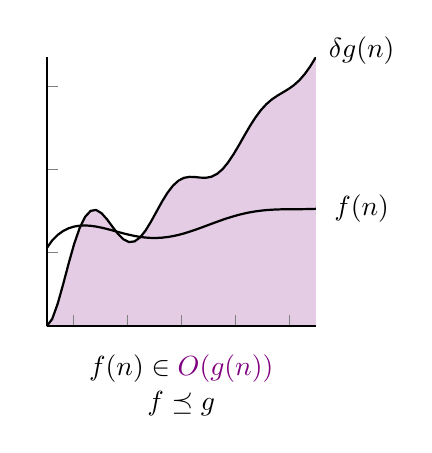
\begin{tikzpicture}
                        \begin{axis}[
                            axis on top=true,
                            axis line style=thick,
                            no markers, domain=1:11, samples=50,
                            axis lines*=left, xlabel=\shortstack{$f(n) \in \violet{O(g(n))}$\\$f \preceq g$}, ylabel=,
                            height=5cm, width=5cm,
                            enlargelimits=false,
                            xticklabels={,,},
                            yticklabels={,,}
                        ]
                            \addplot[fill=violet!20, draw=none] {10 + 0.2*\x^2 + 10*sin(deg(2*(x - 2)))/x} \closedcycle;
                            \addplot[thick] {10 + 0.2*\x^2 + 10*sin(deg(2*(x - 2)))/x};
                            \addplot[thick] {10 + 0.5*\x + 5*sin(deg(x - 1))/x};
                        \end{axis}
                        \node at (4, 3.5) {$\delta g(n)$};
                        \node at (4, 1.5) {$f(n)$};
                    \end{tikzpicture}
                    \hfill
                    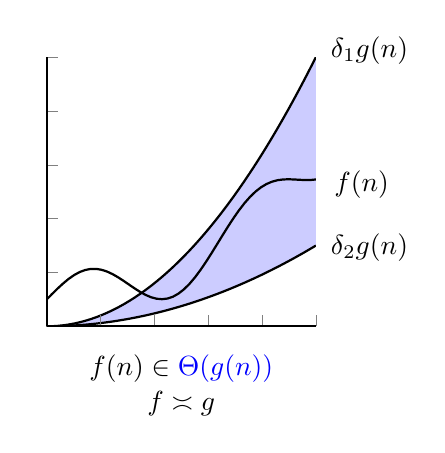
\begin{tikzpicture}
                        \begin{axis}[
                            axis on top=true,
                            axis line style=thick,
                            no markers, domain=0:10, samples=50,
                            axis lines*=left, xlabel=\shortstack{$f(n) \in \blue{\Theta(g(n))}$\\$f \asymp g$}, ylabel=,
                            height=5cm, width=5cm,
                            enlargelimits=false,
                            xticklabels={,,},
                            yticklabels={,,}
                        ]
                            \addplot[fill=blue!20, draw=none] {0.1*\x^2} \closedcycle;
                            \addplot[fill=white, draw=none] {0.03*\x^2} \closedcycle;
                            \addplot[thick] {0.1*\x^2};
                            \addplot[thick] {0.03*\x^2};
                            \addplot[thick] {1 + 0.05*\x^2 + sin(deg(x))};
                        \end{axis}
                        \node at (4.1, 3.5) {$\delta_1 g(n)$};
                        \node at (4.1, 1) {$\delta_2 g(n)$};
                        \node at (4, 1.8) {$f(n)$};
                    \end{tikzpicture}
                    \hfill
                    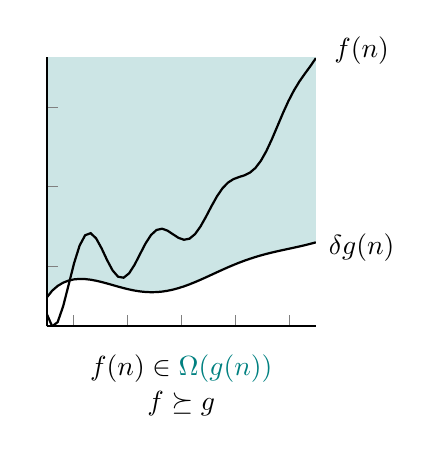
\begin{tikzpicture}
                        \begin{axis}[
                            axis on top=true,
                            axis line style=thick,
                            no markers, domain=1:11, samples=50,
                            axis lines*=left, xlabel=\shortstack{$f(n) \in \teal{\Omega(g(n))}$\\$f \succeq g$}, ylabel=,
                            height=5cm, width=5cm,
                            enlargelimits=false,
                            xticklabels={,,},
                            yticklabels={,,}
                        ]
                            \addplot[fill=teal!20, draw=none] {36.3} \closedcycle;
                            \addplot[fill=white, draw=none] {6 + 0.06*\x^2 + 5*sin(deg(x - 1))/x} \closedcycle;
                            \addplot[thick] {10 + 0.02*\x^3 + 10*sin(deg(2.5*(x - 2)))/x};
                            \addplot[thick] {6 + 0.06*\x^2 + 5*sin(deg(x - 1))/x};
                        \end{axis}
                        \node at (4, 3.5) {$f(n)$};
                        \node at (4, 1) {$\delta g(n)$};
                    \end{tikzpicture}
                \end{center}
                If $f$ and $g$ are L-functions, then either;
                \begin{center}
                    $f \in o(g)$, $f \in \Theta(g)$, or $f \in \Omega(g)$
                \end{center}
                Another method of visualising this is as a Venn diagram, with the upper circle being $O(g(n))$, and the lower circle being $\Omega(g(n))$;
                \begin{center}
                    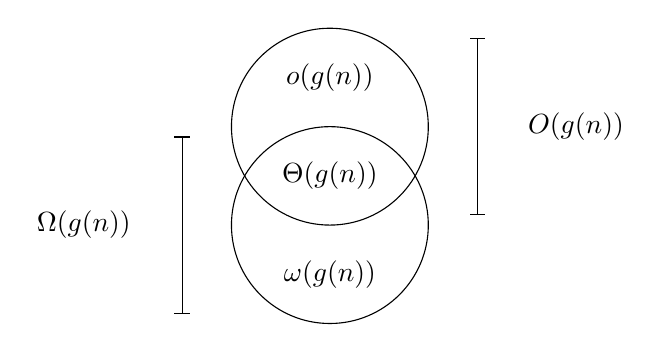
\begin{tikzpicture}[x=1.25cm, y=1.25cm]
                        \draw (0, 0) circle (1);
                        \draw (0, -1) circle (1);
                        \node at (0, 0.5) {$o(g(n))$};
                        \node at (0, -0.5) {$\Theta(g(n))$};
                        \node at (0, -1.5) {$\omega(g(n))$};
                        \node at (2.5, 0) {$O(g(n))$};
                        \node at (-2.5, -1) {$\Omega(g(n))$};
                        \draw
                        (1.5, 0.9) edge[|-|] (1.5, -0.9)
                        (-1.5, -0.1) edge[|-|] (-1.5, -1.9);
                    \end{tikzpicture}
                \end{center}
                Finally, this can also be defined by the following;
                \begin{align*}
                    o(g(n)) & = \{ f \bnfsep \forall \delta > 0.\ \exists n_0 > 0.\ \forall n > n_0.\ |f(n)| < \delta g(n) \} \\
                    O(g(n)) & = \{ f \bnfsep \violet{\exists \delta > 0.\ \exists n_0 > 0.\ \forall n > n_0.\ |f(n)| \leq \delta g(n)} \} \\
                    \Theta(g(n)) & = \left\{f\ \left|\ \begin{matrix}
                        (\violet{\exists \delta > 0.\ \exists n_0 > 0.\ \forall n > n_0.\ |f(n)| \leq \delta g(n)}) \\
                        \land \\
                        (\teal{\exists \delta > 0.\ \forall n_0 > 0.\ \exists n > n_0.\ |f(n)| \geq \delta g(n)})
                    \end{matrix}\right.\right\} \\
                    & = O(g(n)) \cap \Omega(g(n)) \\
                    \Omega(g(n)) & = \{f \bnfsep \teal{\exists \delta > 0.\ \forall n_0 > 0.\ \exists n > n_0.\ |f(n)| \geq \delta g(n)}\} \\
                    \omega(g(n)) & = \{ f \bnfsep \forall \delta > 0.\ \forall n_0 > 0.\ \exists n > n_0.\ |f(n)| > \delta g(n) \}
                \end{align*}
\end{document}
